% 原文 pp.49--55、2.5節導入、2.5.1--2.5.2。
\subsectionlink{測定問題と量子から古典への移行}
この節では、本文ですでに何度か触れた、よくも悪くも有名な量子力学の測定問題を述べる。「測定問題」という用語が選ばれた理由は、純粋に歴史的なものである。測定問題に関連する、ある種の基礎的問題が、系と相互作用する測定装置の量子力学的記述という文脈で、初めて示されたのである。

しかし「測定問題」という用語は、主として次の二つの理由から、範囲が狭すぎるとも考えられる。第一に、以下で見るように、測定問題は異なる三つの問題からなるので、むしろ複数の「測定問題」と言うのが適切だろう。第二に、量子測定と、そこで生じる基礎的問題は、量子から古典への移行という、より一般的な問題の特殊な場合にすぎない。後者は、基礎にある量子的領域から、私たちの周囲の実効的に古典的な系と性質が、どう現れるかという問いである。

したがって一方で、量子から古典への移行の問題は、文字どおりの量子測定の問題より、はるかに広い範囲を持つ。しかし他方で、物理系間の多くの相互作用は、測定に似た相互作用と見なせる。たとえば物体で散乱された光は、物体の位置に関する情報を持ち去るので、この意味で、入射光子を「測定装置」と見なせる。このように遍在する、測定に似た相互作用こそが、デコヒーレンスによる量子から古典への移行の説明の核心にある。より一般的な意味での測定は、量子から古典への移行という広い文脈でも、引き続き最重要の位置を占める。このことが、「測定問題」を完全に捨てて、より一般的な「量子から古典への移行の問題」に置き換えない理由となる。

% 原文 p.50
\hypertarget{srcpage:50}{}\label{srcpage:50}
上に示したように、測定問題、そして量子から古典への移行の問題は、三つの部分からなり、そのすべてを以下でより詳しく述べる。
\begin{enumerate}
\item 優先基底の問題（2.5.2節）。自然界で優先される物理量を、何が選び出すのか。たとえば、なぜ物理系は通常、位置の重ね合わせではなく、確定した位置に観測されるのか。
\item 干渉が観測されない問題（2.5.3節）。特に巨視的尺度で、なぜ量子干渉効果を観測するのは、それほど難しいのか。
\item 結果の問題（2.5.4節）。そもそも、なぜ測定には結果があり、量子確率分布が記述する異なる可能性のうち、何が特定の結果を選ぶのか。
\end{enumerate}
デコヒーレンスの適用範囲、成果、および含意を正しく理解するには、これらの問題に精通することが重要になる。先取りすれば、デコヒーレンスは最初の二つの問題を本質的に解決したと結論するのが、公平である。これらの問題とその解決は、量子力学の標準的形式の内部で、純粋に操作的な言葉で定式化できるので、これら二つに対処する際にデコヒーレンスが果たす役割は、ほとんど争われていない。

これに対し、第三の問題、すなわち結果の問題に取り組むうえでのデコヒーレンスの成功は、なお議論の対象である。特にこの問題は、量子力学の特定の解釈の選択と、ほとんど不可分に結び付いているからである（それは大部分、個人的な好みの問題に帰着する）。実際、デコヒーレンスが「その」測定問題を解けるかについての、過度に楽観的または悲観的な主張の大半は、より解釈的な結果の問題を解決するうえで、デコヒーレンスという標準的な量子効果が持ちうる適用範囲についての、誤解に遡れる。

\subsubsectionlink{理想的量子測定に対するvon Neumannの方式}
二つの別々の、もつれていない系から出発して、もつれた複合状態はどう生じるのだろうか。二つの部分系が個別性を失って、量子力学的な全体となるのは、どうして可能なのか。量子もつれは、重ね合わせ原理という運動学的概念と、Schrödinger時間発展の線形性という力学的性質の組合せから生じると見なせる。その結果としての過程は、しばしばvon Neumann測定として表される。これはvon Neumannが量子力学の初期に考案し、1932年の画期的な著書\cite{ref060}で論じた方式である。

von Neumannの目標は、系だけでなく装置、そして最終的には観測者（9.2節）をも量子力学的対象として扱い、量子測定という行為を、測定される系と測定装置の物理的相互作用として、完全に量子力学の言葉で記述することだった。この方法は、量子力学の法則に従わない、本質的に古典的な測定装置の存在を仮定していたCopenhagen解釈からの、根本的な離脱であったことに注意したい（8.1節）。

% 原文 p.51
\hypertarget{srcpage:51}{}\label{srcpage:51}
その名前にもかかわらず、von Neumann測定方式の適用範囲は、実際の意味での量子測定の文脈を、はるかに超える。実際、von Neumann方式は、量子もつれがどう生じるかを理解する最も容易な方法である。また、上に述べた測定問題の三つの成分、すなわち優先基底の問題、干渉効果が観測されない問題、および結果の問題を、うまく示す。最後に、系と環境の間のvon Neumann型の測定相互作用の帰結としてデコヒーレンスを見なすことにより、その基本的な形式を導入できる。

これらの導入的な注意を踏まえ、von Neumann測定方式を定式化しよう。その典型的な構成要素は、基底ベクトル$\{\lvert s_i\rangle\}$を持つHilbert空間$\mathcal H_{\mathcal S}$で記述される、通常は微視的な系$\mathcal S$と、Hilbert空間$\mathcal H_{\mathcal A}$の基底ベクトル$\{\lvert a_i\rangle\}$で形式的に表される、通常は巨視的な測定装置$\mathcal A$である。厳密に言えば、系と装置が微視的か巨視的かは、以下の一般的議論に影響しない。ただし、系を重ね合わせ状態へ容易に準備できることを確保したいので、物理的には通常、系を微視的なものと結び付けるのが妥当である。他方、測定装置の物理的実現は、通常、多数の自由度を持つ巨視的な系を含む。経験からは、そのような装置は古典物理学の法則に従って振る舞うと期待するだろうが、von Neumann方式は、あえて装置を量子力学的に扱う。

装置の目的は、系$\mathcal S$の状態を測定することである。装置には何らかの指針があり、系が状態$\lvert s_i\rangle$に測定されたとき、状態$\lvert a_i\rangle$で表される位置「$i$」に動くと考えられる（図2.4）。測定前に装置が、初期の「準備完了」状態$\lvert a_r\rangle$から出発すると仮定すれば、系と装置の力学的な測定相互作用は、すべての$i$について
\begin{equation}\lvert s_i\rangle\lvert a_r\rangle\longrightarrow\lvert s_i\rangle\lvert a_i\rangle\tag{2.52}\end{equation}
という形になる。初期状態と終状態は、全系$\mathcal{SA}$を記述するテンソル積Hilbert空間$\mathcal H_{\mathcal S}\otimes\mathcal H_{\mathcal A}$に属する。測定によって、系の状態と装置の状態の間に、一対一の対応が確立されていることが分かる。後者は前者を完全に映している。また式(2.52)の右辺を書く際に、測定相互作用が系の状態を変えないと、暗黙に仮定したことにも注意しよう。これらの仮定により、測定方式(2.52)は、しばしば理想的と呼ばれる。系の状態を乱さないこのような測定は、量子非破壊測定としても知られる\cite{ref069}。

% 原文 p.52
\hypertarget{srcpage:52}{}\label{srcpage:52}
\begin{figure}[htbp]\centering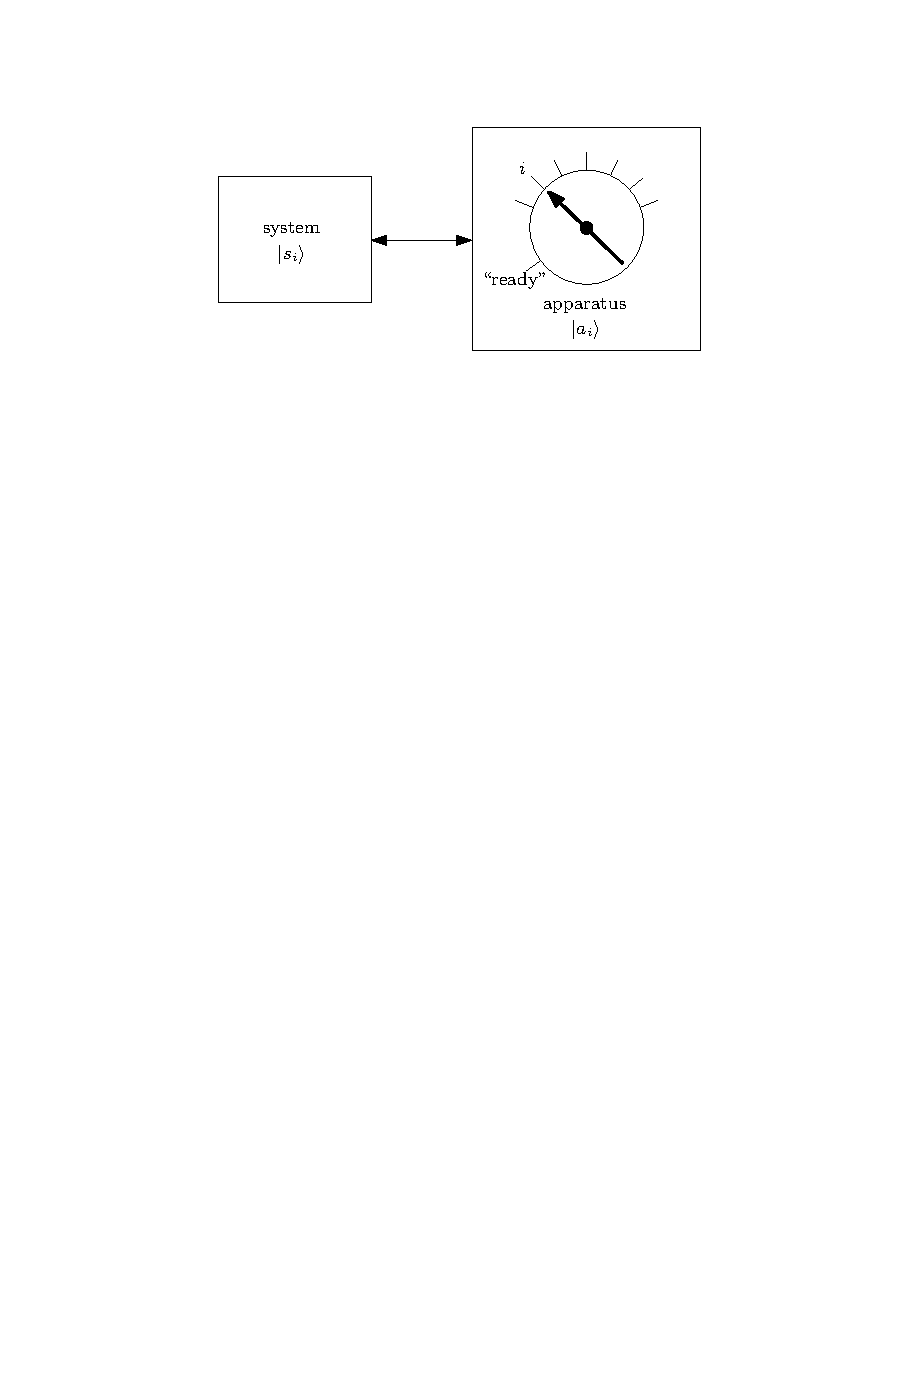
\includegraphics[width=.82\linewidth]{figures/ch02_fig04.pdf}\caption{理想的量子測定に対するvon Neumann方式。系と装置の両方を量子系として扱う。系と装置の相互作用は、系が状態$\lvert s_i\rangle$にあると、装置の指針が、目盛上の初期の「準備完了」位置から、装置の量子状態$\lvert a_i\rangle$で表される位置「$i$」へ動くようなものである。}\end{figure}

ここで重要な点に至る。これまでのところ、相互作用(2.52)は量子もつれを生じていない。系と装置の終状態は、なお分離可能である。しかし、系が初めに基底状態$\lvert s_i\rangle$の重ね合わせ
\begin{equation}\lvert\psi\rangle=\sum_i c_i\lvert s_i\rangle\tag{2.53}\end{equation}
にあるとき、何が起こるかを考えよう。この場合、Schrödinger方程式の線形性によれば、系と装置を合わせた$\mathcal{SA}$は、
\begin{equation}\lvert\psi\rangle\lvert a_r\rangle=\left(\sum_i c_i\lvert s_i\rangle\right)\lvert a_r\rangle\longrightarrow\lvert\Psi\rangle=\sum_i c_i\lvert s_i\rangle\lvert a_i\rangle\tag{2.54}\end{equation}
に従って発展する。この発展が、理想的なvon Neumann量子測定方式を表す。

式(2.54)の右辺を調べると、系と装置の組合せの終状態は、一般にもつれ状態で記述されることが分かる。すなわち、もはや系や装置に個別の状態ベクトルを帰属させられない。こうして量子もつれが力学的に作り出された。初めは系だけに存在した重ね合わせは、最終的な重ね合わせが系と装置の両方を含むという意味で、通常巨視的な装置の水準へ増幅された。

ここで決定的な難点は、式(2.54)が記述する力学的発展を、通常の意味の測定を表すと、どう見なすべきかが、まったく明らかでないことである。というのも、以下で論じる少なくとも二つの理由から、式(2.54)の右辺の終状態だけでは、測定が実際に完了したと直接に結論するのに不十分だからである。この事実を強調するため、方式(2.54)は、しばしば前測定と呼ばれる。

% 原文 p.53
\hypertarget{srcpage:53}{}\label{srcpage:53}
\subsubsectionlink{優先基底の問題}
第一の問題は、式(2.54)の右辺の最終的な複合状態の展開について、基底の曖昧さが存在することである。この状態は多くの異なる方法で表せるので、上のvon Neumann方式で測定されたはずの観測可能量は、この終状態によって一意には定義されない。実際、系$\mathcal S$を記述する任意の状態の組が与えられると、最終的な複合状態が式(2.54)の形を取るような、対応する装置状態の組が存在する。
\begin{equation}\lvert\psi\rangle\lvert a_r\rangle\longrightarrow\lvert\Psi\rangle=\sum_i c_i\lvert s_i\rangle\lvert a_i\rangle=\sum_i c_i'\lvert s_i'\rangle\lvert a_i'\rangle=\cdots.\tag{2.55}\end{equation}
しかし、基底選択のこの自由は、実際には二つの制約によって、ある程度制限される。第一に、通常は装置の状態$\lvert a_i\rangle$が互いに直交することを要求する。これにより、これらの状態が古典的に異なる測定結果に対応し、系の可能な状態$\lvert s_i\rangle$を確実に識別できる。第二に、装置状態の組$\lvert a_i\rangle$を任意に選ぶと、系の相対状態$\lvert s_i\rangle$は、互いに直交しないかもしれない。その場合、状態$\lvert s_i\rangle$に対応する、すなわち、それらを固有状態とする系の観測可能量は、Hermiteにならず、これは通常望ましくない性質である\footnote{ただし、非Hermiteな観測可能量は、先験的に禁止されているわけではなく、ある実験設定では現れる。たとえば量子光学では、コヒーレント状態を結果とする測定をしばしば行う。しかしコヒーレント状態は過完備な組をなし、したがってHermiteな観測可能量では表せない。Zurekの議論\cite{ref016}も参照。}。

これらを踏まえ、装置状態$\lvert a_i\rangle$は互いに直交し、すなわち$i\ne j$で$\langle a_i\vert a_j\rangle=0$と要求してよい。この場合、いわゆるSchmidt定理（後の2.15.1節）から、分解
\begin{equation}\lvert\Psi\rangle=\sum_i c_i\lvert s_i\rangle\lvert a_i\rangle,\qquad c_i\in\mathbb R,\quad\sum_i c_i^2=1\tag{2.56}\end{equation}
は、すべての係数$c_i$が互いに異なる限り、一意であることが従う。

% 原文 p.54
\hypertarget{srcpage:54}{}\label{srcpage:54}
係数についてのこの条件が成り立たないと、分解(2.56)が一般に一意ではないことを示す、単純な例を考えよう。系$\mathcal S$と装置$\mathcal A$が、どちらもスピン$1/2$粒子で表される量子力学的二状態系であり、基底状態$\lvert0_z\rangle$、$\lvert1_z\rangle$で記述されるとする。さらに、$\mathcal A$の状態$\lvert0_z\rangle_{\mathcal A}$、$\lvert1_z\rangle_{\mathcal A}$が、$\mathcal S$のスピン状態$\lvert0_z\rangle_{\mathcal S}$、$\lvert1_z\rangle_{\mathcal S}$の「指針」として働くとする。つまり、ここでのvon Neumann相互作用(2.52)は、
\begin{equation}\begin{split}\lvert0_z\rangle_{\mathcal S}\lvert\text{「準備完了」}\rangle_{\mathcal A}&\longrightarrow\lvert0_z\rangle_{\mathcal S}\lvert0_z\rangle_{\mathcal A},\\\lvert1_z\rangle_{\mathcal S}\lvert\text{「準備完了」}\rangle_{\mathcal A}&\longrightarrow\lvert1_z\rangle_{\mathcal S}\lvert1_z\rangle_{\mathcal A}\end{split}\tag{2.57}\end{equation}
という力学で記述される。系$\mathcal S$が重ね合わせ$(\lvert0_z\rangle_{\mathcal S}+\lvert1_z\rangle_{\mathcal S})/\sqrt2$から出発すると仮定すれば、式(2.57)とSchrödinger方程式の線形性から［式(2.54)も参照］、最終的な、もつれたスピンと装置の複合状態は、
\begin{equation}\lvert\Psi\rangle=\frac1{\sqrt2}(\lvert0_z\rangle_{\mathcal S}\lvert0_z\rangle_{\mathcal A}+\lvert1_z\rangle_{\mathcal S}\lvert1_z\rangle_{\mathcal A})\tag{2.58}\end{equation}
となる。式(2.35)を用いて、$z$スピン状態$\lvert0_z\rangle_i$、$\lvert1_z\rangle_i$（$i=\mathcal S,\mathcal A$）を、Pauliスピン演算子$\hat\sigma_x$の固有状態$\lvert0_x\rangle_i$、$\lvert1_x\rangle_i$で書き直そう。新しい基底$\{\lvert0_x\rangle_i,\lvert1_x\rangle_i\}$で表すと、状態(2.58)は
\begin{equation}\lvert\Psi\rangle=\frac1{\sqrt2}(\lvert0_x\rangle_{\mathcal S}\lvert0_x\rangle_{\mathcal A}+\lvert1_x\rangle_{\mathcal S}\lvert1_x\rangle_{\mathcal A})\tag{2.59}\end{equation}
となる。$\mathcal A$を、系$\mathcal S$のスピンの測定装置と見なしたことを思い出そう。式(2.58)、(2.59)は、装置$\mathcal A$が、$\mathcal S$の$z$スピン状態とも$x$スピン状態とも、一対一の相関を作ったことを意味する。von Neumann方式の精神に従い、その後の波動関数の収縮を仮定せず、系と装置の相関形成を完全な測定と解釈すると、この状況は次を意味するように見える。$\mathcal A$が$\mathcal S$の$z$軸方向のスピンを測定した時点で［終状態(2.58)］、$\mathcal S$の$x$軸方向のスピンも測定したと見なせる。後者の「測定」は、式(2.58)の同値な形(2.59)で表される。

したがって装置$\mathcal A$は、系の二つの非可換な観測可能量、すなわち$\hat\sigma_x$と$\hat\sigma_z$を同時に測定したように見え、量子力学の法則に反するように思われる。さらに、状態(2.58)は、実際には任意の軸に沿ったスピン$1/2$の基底を用いて、無限通りの同値な方法で書き直せると容易に示せる。したがって、装置$\mathcal A$が、式(2.58)の型の相関の形成というvon Neumannの意味で、$\mathcal S$の$z$軸方向のスピンを「測定」した時点で、他のすべての空間方向のスピンも「測定」したように見える。

非可換な観測可能量の組を同時に測定するこの状況は、量子力学で禁止されるだけでなく、測定装置はごく特定の量だけを測定するよう設計されているという経験にも反する。この例では、装置$\mathcal A$をStern--Gerlach装置（2.2.2節）として実現でき、状態$\lvert0_z\rangle_{\mathcal A}$、$\lvert1_z\rangle_{\mathcal A}$は、$z$軸方向に磁場を向けた装置を通る、分離した二つの経路に対応し、それによって系$\mathcal S$のスピン状態$\lvert0_z\rangle_{\mathcal S}$、$\lvert1_z\rangle_{\mathcal S}$を区別する。したがって、このStern--Gerlach装置は、$z$軸方向だけのスピンを測り、他の軸方向は測らないように設定されている。$z$と異なる軸に沿って測定するには、磁場を物理的に回転させる必要があり、物理的に異なる設定に対応する。

% 原文 p.55
\hypertarget{srcpage:55}{}\label{srcpage:55}
このような「優先観測可能量」、あるいは「優先基底」の存在は、von Neumann測定で到達する、系と装置の終状態では説明されない。見たように、この状態の形は一般に、量子的相関の形成を介して装置が記録する系の観測可能量を一意には固定しない。この優先基底の問題を、波動関数収縮の問題、およびそれと密接に関係する結果の問題（後の2.5.4節）から初めて明瞭に切り離したのはZurek\cite{ref008}であり、量子測定のいかなる説明でも優先基底の問題が果たす、独立した重要な役割を強調した。可能な結果の集合が明確に定義されていなければ、特定の結果を問うことさえ意味を持たないので、結果の問題が役割を持つ以前に、この優先基底の問題を解く必要がある。

Zurekはまた\cite{ref008,ref009}、優先基底の問題が、量子測定という狭い文脈をはるかに超えて、量子から古典への移行の問題で中心的役割を果たすことを認識した。ここでは、なぜ系、特に巨視的な系を、重ね合わせ原理が原理上許す物理量の、ごく小さな部分集合でしか知覚しないのか、という核心的な問いに出会う。最も顕著な例として、巨視的な系は常に、位置の重ね合わせではなく、確定した空間位置に見いだされる。何が位置を優先される量として選び出すのか。Zeh\cite{ref004}が最初に示唆し、Zurek\cite{ref008,ref009}が詳細に述べたように、これらに答え、優先基底の問題を克服するには、系と装置を、環境と相互作用する開いた量子系として考えなければならない。この方法を2.8節で詳しく論じる。
